\section{Methodology}

This section describes the data collection pipeline and the overall approach used in
Geo-SLM. The data subsection covers the construction of the training dataset from raw
academic papers. The approach subsection presents the 5-stage hybrid pipeline architecture.

% ============================================================
\subsection{Data}
% ============================================================

\subsubsection{Data Collection Pipeline}

The training data is collected from approximately 4,000 academic papers in the cs.CV,
cs.LG, and cs.AI categories on arXiv. The collection pipeline transforms raw PDFs into
a structured SLM training dataset through six sequential stages, as illustrated in
\Cref{fig:data_pipeline}.

\begin{figure}[htbp]
\centering
% TikZ: Data Collection Pipeline Flow
% Usage: % TikZ: Data Collection Pipeline Flow
% Usage: % TikZ: Data Collection Pipeline Flow
% Usage: \input{figures/tikz/tikz_data_pipeline.tex}
% Requires: \usepackage{tikz} \usetikzlibrary{shapes.geometric, arrows.meta, positioning, fit, backgrounds}

\begin{tikzpicture}[
    node distance=0.5cm and 0.4cm,
    step/.style={
        rectangle, rounded corners=3pt, draw=#1!60!black, thick,
        minimum width=2.4cm, minimum height=1.0cm,
        fill=#1!12, font=\scriptsize\bfseries, align=center
    },
    count/.style={
        font=\tiny\bfseries, text=#1!70!black, align=center
    },
    arrow/.style={-{Stealth[length=2.5mm]}, thick, draw=black!50},
    filter/.style={font=\tiny\itshape, text=red!60, align=center}
]

% Row 1
\node[step=blue] (arxiv) {arXiv API\\Collection};
\node[step=teal, right=of arxiv] (pdf) {PDF Page\\Extraction};
\node[step=orange, right=of pdf] (yolo) {YOLO\\Detection};

% Row 2
\node[step=purple, right=of yolo] (filter) {Quality\\Filtering};
\node[step=red, below=0.8cm of filter] (classify) {ResNet-18\\Classification};
\node[step=teal, left=of classify] (s3) {Stage 3\\Extraction};

% Row 3
\node[step=blue, left=of s3] (qa) {Gemini QA\\Generation};
\node[step=orange, left=of qa] (dataset) {v3 Dataset\\Assembly};

% Counts
\node[count=blue, below=0.08cm of arxiv] {$\sim$4,000 PDFs};
\node[count=teal, below=0.08cm of pdf] {$\sim$150K pages};
\node[count=orange, below=0.08cm of yolo] {$\sim$70K crops};
\node[count=purple, below=0.08cm of filter] {46,910};
\node[count=red, above=0.08cm of classify] {32,364 charts};
\node[count=teal, above=0.08cm of s3] {32,364 features};
\node[count=blue, above=0.08cm of qa] {291K QA pairs};
\node[count=orange, above=0.08cm of dataset] {268,799 samples};

% Arrows
\draw[arrow] (arxiv) -- (pdf);
\draw[arrow] (pdf) -- (yolo);
\draw[arrow] (yolo) -- (filter);
\draw[arrow] (filter) -- (classify);
\draw[arrow] (classify) -- (s3);
\draw[arrow] (s3) -- (qa);
\draw[arrow] (qa) -- (dataset);

% Filter annotations
\node[filter, above=0.2cm of filter.north west, anchor=south west] {min res, dedup,\\non-chart removal};

\end{tikzpicture}

% Requires: \usepackage{tikz} \usetikzlibrary{shapes.geometric, arrows.meta, positioning, fit, backgrounds}

\begin{tikzpicture}[
    node distance=0.5cm and 0.4cm,
    step/.style={
        rectangle, rounded corners=3pt, draw=#1!60!black, thick,
        minimum width=2.4cm, minimum height=1.0cm,
        fill=#1!12, font=\scriptsize\bfseries, align=center
    },
    count/.style={
        font=\tiny\bfseries, text=#1!70!black, align=center
    },
    arrow/.style={-{Stealth[length=2.5mm]}, thick, draw=black!50},
    filter/.style={font=\tiny\itshape, text=red!60, align=center}
]

% Row 1
\node[step=blue] (arxiv) {arXiv API\\Collection};
\node[step=teal, right=of arxiv] (pdf) {PDF Page\\Extraction};
\node[step=orange, right=of pdf] (yolo) {YOLO\\Detection};

% Row 2
\node[step=purple, right=of yolo] (filter) {Quality\\Filtering};
\node[step=red, below=0.8cm of filter] (classify) {ResNet-18\\Classification};
\node[step=teal, left=of classify] (s3) {Stage 3\\Extraction};

% Row 3
\node[step=blue, left=of s3] (qa) {Gemini QA\\Generation};
\node[step=orange, left=of qa] (dataset) {v3 Dataset\\Assembly};

% Counts
\node[count=blue, below=0.08cm of arxiv] {$\sim$4,000 PDFs};
\node[count=teal, below=0.08cm of pdf] {$\sim$150K pages};
\node[count=orange, below=0.08cm of yolo] {$\sim$70K crops};
\node[count=purple, below=0.08cm of filter] {46,910};
\node[count=red, above=0.08cm of classify] {32,364 charts};
\node[count=teal, above=0.08cm of s3] {32,364 features};
\node[count=blue, above=0.08cm of qa] {291K QA pairs};
\node[count=orange, above=0.08cm of dataset] {268,799 samples};

% Arrows
\draw[arrow] (arxiv) -- (pdf);
\draw[arrow] (pdf) -- (yolo);
\draw[arrow] (yolo) -- (filter);
\draw[arrow] (filter) -- (classify);
\draw[arrow] (classify) -- (s3);
\draw[arrow] (s3) -- (qa);
\draw[arrow] (qa) -- (dataset);

% Filter annotations
\node[filter, above=0.2cm of filter.north west, anchor=south west] {min res, dedup,\\non-chart removal};

\end{tikzpicture}

% Requires: \usepackage{tikz} \usetikzlibrary{shapes.geometric, arrows.meta, positioning, fit, backgrounds}

\begin{tikzpicture}[
    node distance=0.5cm and 0.4cm,
    step/.style={
        rectangle, rounded corners=3pt, draw=#1!60!black, thick,
        minimum width=2.4cm, minimum height=1.0cm,
        fill=#1!12, font=\scriptsize\bfseries, align=center
    },
    count/.style={
        font=\tiny\bfseries, text=#1!70!black, align=center
    },
    arrow/.style={-{Stealth[length=2.5mm]}, thick, draw=black!50},
    filter/.style={font=\tiny\itshape, text=red!60, align=center}
]

% Row 1
\node[step=blue] (arxiv) {arXiv API\\Collection};
\node[step=teal, right=of arxiv] (pdf) {PDF Page\\Extraction};
\node[step=orange, right=of pdf] (yolo) {YOLO\\Detection};

% Row 2
\node[step=purple, right=of yolo] (filter) {Quality\\Filtering};
\node[step=red, below=0.8cm of filter] (classify) {ResNet-18\\Classification};
\node[step=teal, left=of classify] (s3) {Stage 3\\Extraction};

% Row 3
\node[step=blue, left=of s3] (qa) {Gemini QA\\Generation};
\node[step=orange, left=of qa] (dataset) {v3 Dataset\\Assembly};

% Counts
\node[count=blue, below=0.08cm of arxiv] {$\sim$4,000 PDFs};
\node[count=teal, below=0.08cm of pdf] {$\sim$150K pages};
\node[count=orange, below=0.08cm of yolo] {$\sim$70K crops};
\node[count=purple, below=0.08cm of filter] {46,910};
\node[count=red, above=0.08cm of classify] {32,364 charts};
\node[count=teal, above=0.08cm of s3] {32,364 features};
\node[count=blue, above=0.08cm of qa] {291K QA pairs};
\node[count=orange, above=0.08cm of dataset] {268,799 samples};

% Arrows
\draw[arrow] (arxiv) -- (pdf);
\draw[arrow] (pdf) -- (yolo);
\draw[arrow] (yolo) -- (filter);
\draw[arrow] (filter) -- (classify);
\draw[arrow] (classify) -- (s3);
\draw[arrow] (s3) -- (qa);
\draw[arrow] (qa) -- (dataset);

% Filter annotations
\node[filter, above=0.2cm of filter.north west, anchor=south west] {min res, dedup,\\non-chart removal};

\end{tikzpicture}

\caption{Data collection pipeline: from arXiv papers to SLM training dataset.
    Each stage filters and transforms the data, reducing volume while increasing quality.}
\label{fig:data_pipeline}
\end{figure}

\Cref{tab:data_scale} summarizes the scale at each stage of the pipeline.

\begin{table}[htbp]
\centering
\caption{Data pipeline scale at each processing stage.}
\label{tab:data_scale}
\begin{table}[htbp]
\centering
\caption{Data Collection Pipeline Scale}
\label{tab:data-pipeline-scale}
\begin{tabular}{@{}lr@{}}
\toprule
\textbf{Stage} & \textbf{Count} \\
\midrule
arXiv PDFs processed      &  $\sim$4,000 \\
Raw page images           & $\sim$150,000 \\
Candidate chart regions   &  $\sim$70,000 \\
After quality filtering   &     46,910 \\
Final classified charts   &     32,364 \\
OCR cache entries         &     46,910 \\
SLM training samples (v3) &    268,799 \\
\bottomrule
\end{tabular}
\end{table}
\end{table}

\textbf{Step 1: PDF Mining.}
PyMuPDF renders each PDF page at 150~DPI, producing approximately 150,000 page images.
The ArXiv API is accessed with rate limiting ($\sim$3s between requests) and resume
capability via progress files.

\textbf{Step 2: Chart Detection.}
A trained YOLOv8m model (confidence threshold 0.5) detects chart regions in each page
image, yielding approximately 70,000 candidate chart crops.

\textbf{Step 3: Classification and Filtering.}
A cascade classifier (ResNet-18 primary, rule-based fallback) assigns each crop to one
of 8 chart types: line, bar, scatter, pie, histogram, box, heatmap, and area. After
filtering low-confidence detections and duplicates, 32,364 verified charts remain.
\Cref{tab:chart_dist} shows the distribution by type.

\begin{table}[htbp]
\centering
\caption{Chart type distribution in the classified dataset (32,364 charts).}
\label{tab:chart_dist}
\begin{tabular}{@{}lrr@{}}
\toprule
\textbf{Chart Type} & \textbf{Count} & \textbf{Share (\%)} \\
\midrule
line      & 10,036 & 31.0 \\
bar       &  9,086 & 28.1 \\
box       &  4,867 & 15.0 \\
scatter   &  2,802 &  8.7 \\
pie       &  2,421 &  7.5 \\
histogram &  2,060 &  6.4 \\
heatmap   &    680 &  2.1 \\
area      &    412 &  1.3 \\
\midrule
\textbf{Total} & \textbf{32,364} & \textbf{100.0} \\
\bottomrule
\end{tabular}
\end{table}

\textbf{Step 4: Feature Extraction.}
The Stage~3 extraction pipeline (see \Cref{sec:system_s3}) processes all 32,364 charts
using parallel batch execution. The extraction achieves 100\% success rate with 0\%
data corruption, producing structured feature JSONs containing axis calibration,
OCR text with spatial roles, detected elements, and confidence scores.

\textbf{Step 5: QA Generation.}
The \texttt{data\_factory} tool uses Gemini 2.0 Flash API to generate 10 questions per
chart across four difficulty levels: shallow (25\%), intermediate (35\%), deep (30\%),
and conceptual (10\%). This produces approximately 291,000 QA pairs. Cross-validation
confirms 87\% text overlap between Stage~3 features and QA answers.

\textbf{Step 6: Dataset Assembly.}
The final SLM training dataset (v3) is assembled by merging Stage~3 features with QA
pairs, formatted as ChatML conversations. The dataset is split by \texttt{chart\_id}
to prevent data leakage between train, validation, and test sets.

\subsubsection{SLM Training Dataset}

\Cref{tab:splits} shows the dataset split statistics.

\begin{table}[htbp]
\centering
\caption{SLM training dataset v3 split statistics.}
\label{tab:splits}
\begin{tabular}{@{}lrr@{}}
\toprule
\textbf{Split} & \textbf{Samples} & \textbf{Ratio (\%)} \\
\midrule
Train      & 228,494 & 85 \\
Validation &  26,888 & 10 \\
Test       &  13,417 &  5 \\
\midrule
\textbf{Total} & \textbf{268,799} & \textbf{100} \\
\bottomrule
\end{tabular}
\end{table}

The v3 dataset represents a 9.9$\times$ improvement over v2 (27,159 $\to$ 268,799
samples), achieved by fixing axis key format errors (coverage increased from 4\%
to 69.9\%), ensuring 100\% Stage~3 feature coverage, and implementing chart-ID-based
splitting to eliminate data leakage.

\Cref{fig:data_funnel} visualizes the data reduction funnel across pipeline stages.

\begin{figure}[htbp]
\centering
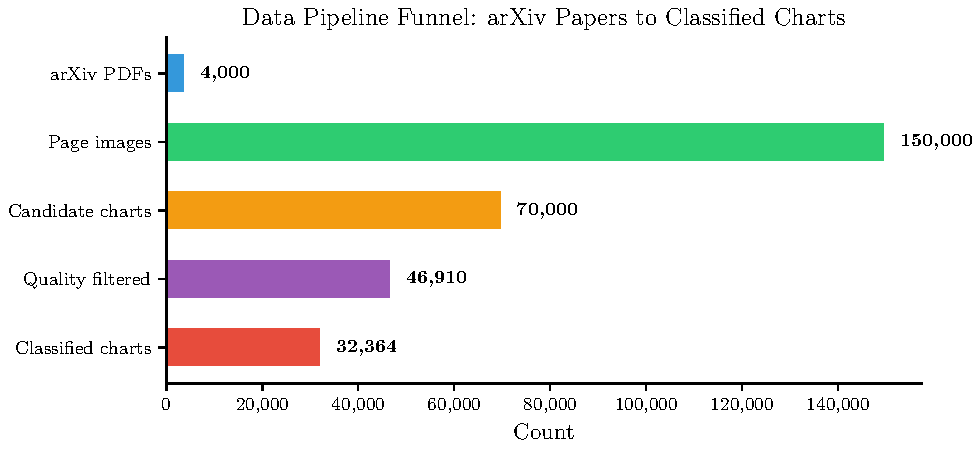
\includegraphics[width=0.85\textwidth]{figures/fig_data_pipeline_funnel.pdf}
\caption{Data pipeline funnel: volume at each stage from raw PDFs to final dataset.}
\label{fig:data_funnel}
\end{figure}

\subsubsection{SLM Fine-Tuning Configuration}

The SLM is fine-tuned using QLoRA \cite{dettmers2024qlora} on the Qwen-2.5-1.5B-Instruct
base model \cite{yang2024qwen2}. \Cref{tab:slm_config} lists the training hyperparameters.

\begin{table}[htbp]
\centering
\caption{SLM fine-tuning configuration (QLoRA).}
\label{tab:slm_config}
\begin{tabular}{@{}ll@{}}
\toprule
\textbf{Parameter} & \textbf{Value} \\
\midrule
Base model       & Llama-3.2-1B-Instruct \\
Method           & QLoRA (4-bit NF4 + LoRA rank 16) \\
LoRA targets     & q, k, v, o, gate, up, down projections \\
Optimizer        & paged\_adamw\_32bit \\
LR scheduler     & Cosine (warmup 5\%) \\
VRAM requirement & $\sim$4--5 GB (RTX 3060 6GB) \\
Batch size       & 2 (effective 16 with gradient accumulation 8) \\
Learning rate    & $2 \times 10^{-4}$ \\
Max seq.\ length & 1024 tokens \\
Precision        & bf16 (mixed precision) \\
Weight decay     & 0.01 \\
LoRA dropout     & 0.05 \\
\bottomrule
\end{tabular}
\end{table}

The QLoRA configuration uses 4-bit NF4 quantization with LoRA rank~16, resulting in
11.27M trainable parameters (0.9\% of total). This fits within the 6~GB VRAM constraint
of an NVIDIA RTX~3060. Training follows a 4-stage curriculum: (1) chart type and axis
labels, (2) value extraction and OCR correction, (3) trends and comparisons, and
(4) noisy OCR and complex layouts.

% ============================================================
\subsection{Approach}
% ============================================================

\subsubsection{Hybrid Neuro-Symbolic Design}

The core hypothesis of Geo-SLM is that treating charts as \textbf{geometric entities}
rather than pixel patterns yields higher extraction accuracy than pure end-to-end
multimodal approaches. The system combines three complementary paradigms:

\begin{itemize}
    \item \textbf{Deep Learning} for perception: detecting chart regions (YOLOv8) and
          classifying chart types (ResNet-18).
    \item \textbf{Symbolic/Geometric Analysis} for precision: calibrating axes (RANSAC),
          simplifying curves (RDP), and mapping pixel coordinates to data values.
    \item \textbf{Language Model Reasoning} for understanding: correcting OCR errors,
          validating extracted data, and generating natural language descriptions.
\end{itemize}

\Cref{fig:approach_cmp} contrasts the traditional end-to-end approach with the Geo-SLM
hybrid approach.

\begin{figure}[htbp]
\centering
% TikZ: Hybrid Approach Comparison (Traditional vs Geo-SLM)
% Usage: % TikZ: Hybrid Approach Comparison (Traditional vs Geo-SLM)
% Usage: % TikZ: Hybrid Approach Comparison (Traditional vs Geo-SLM)
% Usage: \input{figures/tikz/tikz_approach_comparison.tex}
% Requires: \usepackage{tikz} \usetikzlibrary{shapes.geometric, arrows.meta, positioning, fit, backgrounds, calc}

\begin{tikzpicture}[
    node distance=0.4cm and 0.6cm,
    block/.style={
        rectangle, rounded corners=2pt, draw=black!60, thick,
        minimum width=2.0cm, minimum height=0.8cm,
        font=\scriptsize\bfseries, align=center
    },
    arrow/.style={-{Stealth[length=2.5mm]}, thick, draw=black!50},
    grouplabel/.style={font=\small\bfseries, text=black!70},
    prob/.style={font=\tiny\itshape, text=red!60},
    good/.style={font=\tiny\itshape, text=teal!70}
]

% Traditional approach (top)
\node[grouplabel] (trad_label) at (0, 2.5) {(a) Traditional End-to-End};

\node[block, fill=blue!15] (t_img) at (0, 1.6) {Chart\\Image};
\node[block, fill=red!15, right=of t_img] (t_llm) {Multimodal\\LLM};
\node[block, fill=yellow!15, right=of t_llm] (t_text) {Text\\Description};
\node[block, fill=gray!15, right=of t_text] (t_parse) {Parse\\to Data};

\draw[arrow] (t_img) -- (t_llm);
\draw[arrow] (t_llm) -- (t_text);
\draw[arrow] (t_text) -- (t_parse);

\node[prob, below=0.05cm of t_llm] {Hallucination risk};
\node[prob, below=0.05cm of t_text] {Approximate values};

% Geo-SLM approach (bottom)
\node[grouplabel] at (0, 0.3) {(b) Geo-SLM Hybrid};

\node[block, fill=blue!15] (g_img) at (0, -0.6) {Chart\\Image};
\node[block, fill=teal!15, right=of g_img] (g_yolo) {YOLO\\Detection};
\node[block, fill=green!15, right=of g_yolo] (g_geo) {Geometric\\Analysis};
\node[block, fill=orange!15, right=of g_geo] (g_coord) {Measured\\Coordinates};
\node[block, fill=purple!15, right=of g_coord] (g_slm) {SLM\\Refinement};

\draw[arrow] (g_img) -- (g_yolo);
\draw[arrow] (g_yolo) -- (g_geo);
\draw[arrow] (g_geo) -- (g_coord);
\draw[arrow] (g_coord) -- (g_slm);

\node[good, below=0.05cm of g_geo] {Deterministic};
\node[good, below=0.05cm of g_coord] {Traceable};
\node[good, below=0.05cm of g_slm] {1.5B params};

% Divider
\draw[dashed, black!30] (-1.2, 0.9) -- (12, 0.9);

\end{tikzpicture}

% Requires: \usepackage{tikz} \usetikzlibrary{shapes.geometric, arrows.meta, positioning, fit, backgrounds, calc}

\begin{tikzpicture}[
    node distance=0.4cm and 0.6cm,
    block/.style={
        rectangle, rounded corners=2pt, draw=black!60, thick,
        minimum width=2.0cm, minimum height=0.8cm,
        font=\scriptsize\bfseries, align=center
    },
    arrow/.style={-{Stealth[length=2.5mm]}, thick, draw=black!50},
    grouplabel/.style={font=\small\bfseries, text=black!70},
    prob/.style={font=\tiny\itshape, text=red!60},
    good/.style={font=\tiny\itshape, text=teal!70}
]

% Traditional approach (top)
\node[grouplabel] (trad_label) at (0, 2.5) {(a) Traditional End-to-End};

\node[block, fill=blue!15] (t_img) at (0, 1.6) {Chart\\Image};
\node[block, fill=red!15, right=of t_img] (t_llm) {Multimodal\\LLM};
\node[block, fill=yellow!15, right=of t_llm] (t_text) {Text\\Description};
\node[block, fill=gray!15, right=of t_text] (t_parse) {Parse\\to Data};

\draw[arrow] (t_img) -- (t_llm);
\draw[arrow] (t_llm) -- (t_text);
\draw[arrow] (t_text) -- (t_parse);

\node[prob, below=0.05cm of t_llm] {Hallucination risk};
\node[prob, below=0.05cm of t_text] {Approximate values};

% Geo-SLM approach (bottom)
\node[grouplabel] at (0, 0.3) {(b) Geo-SLM Hybrid};

\node[block, fill=blue!15] (g_img) at (0, -0.6) {Chart\\Image};
\node[block, fill=teal!15, right=of g_img] (g_yolo) {YOLO\\Detection};
\node[block, fill=green!15, right=of g_yolo] (g_geo) {Geometric\\Analysis};
\node[block, fill=orange!15, right=of g_geo] (g_coord) {Measured\\Coordinates};
\node[block, fill=purple!15, right=of g_coord] (g_slm) {SLM\\Refinement};

\draw[arrow] (g_img) -- (g_yolo);
\draw[arrow] (g_yolo) -- (g_geo);
\draw[arrow] (g_geo) -- (g_coord);
\draw[arrow] (g_coord) -- (g_slm);

\node[good, below=0.05cm of g_geo] {Deterministic};
\node[good, below=0.05cm of g_coord] {Traceable};
\node[good, below=0.05cm of g_slm] {1.5B params};

% Divider
\draw[dashed, black!30] (-1.2, 0.9) -- (12, 0.9);

\end{tikzpicture}

% Requires: \usepackage{tikz} \usetikzlibrary{shapes.geometric, arrows.meta, positioning, fit, backgrounds, calc}

\begin{tikzpicture}[
    node distance=0.4cm and 0.6cm,
    block/.style={
        rectangle, rounded corners=2pt, draw=black!60, thick,
        minimum width=2.0cm, minimum height=0.8cm,
        font=\scriptsize\bfseries, align=center
    },
    arrow/.style={-{Stealth[length=2.5mm]}, thick, draw=black!50},
    grouplabel/.style={font=\small\bfseries, text=black!70},
    prob/.style={font=\tiny\itshape, text=red!60},
    good/.style={font=\tiny\itshape, text=teal!70}
]

% Traditional approach (top)
\node[grouplabel] (trad_label) at (0, 2.5) {(a) Traditional End-to-End};

\node[block, fill=blue!15] (t_img) at (0, 1.6) {Chart\\Image};
\node[block, fill=red!15, right=of t_img] (t_llm) {Multimodal\\LLM};
\node[block, fill=yellow!15, right=of t_llm] (t_text) {Text\\Description};
\node[block, fill=gray!15, right=of t_text] (t_parse) {Parse\\to Data};

\draw[arrow] (t_img) -- (t_llm);
\draw[arrow] (t_llm) -- (t_text);
\draw[arrow] (t_text) -- (t_parse);

\node[prob, below=0.05cm of t_llm] {Hallucination risk};
\node[prob, below=0.05cm of t_text] {Approximate values};

% Geo-SLM approach (bottom)
\node[grouplabel] at (0, 0.3) {(b) Geo-SLM Hybrid};

\node[block, fill=blue!15] (g_img) at (0, -0.6) {Chart\\Image};
\node[block, fill=teal!15, right=of g_img] (g_yolo) {YOLO\\Detection};
\node[block, fill=green!15, right=of g_yolo] (g_geo) {Geometric\\Analysis};
\node[block, fill=orange!15, right=of g_geo] (g_coord) {Measured\\Coordinates};
\node[block, fill=purple!15, right=of g_coord] (g_slm) {SLM\\Refinement};

\draw[arrow] (g_img) -- (g_yolo);
\draw[arrow] (g_yolo) -- (g_geo);
\draw[arrow] (g_geo) -- (g_coord);
\draw[arrow] (g_coord) -- (g_slm);

\node[good, below=0.05cm of g_geo] {Deterministic};
\node[good, below=0.05cm of g_coord] {Traceable};
\node[good, below=0.05cm of g_slm] {1.5B params};

% Divider
\draw[dashed, black!30] (-1.2, 0.9) -- (12, 0.9);

\end{tikzpicture}

\caption{Comparison of traditional end-to-end approach (top) vs.\ Geo-SLM hybrid
    neuro-symbolic approach (bottom). Geo-SLM uses geometric measurement for precision
    and SLM reasoning for semantic understanding.}
\label{fig:approach_cmp}
\end{figure}

\subsubsection{5-Stage Pipeline Architecture}

The system is organized as a modular 5-stage pipeline where each stage has well-defined
input and output schema contracts (Pydantic v2 frozen models). \Cref{fig:pipeline_arch}
shows the pipeline architecture.

\begin{figure}[htbp]
\centering
% TikZ: 5-Stage Pipeline Architecture
% Usage: % TikZ: 5-Stage Pipeline Architecture
% Usage: % TikZ: 5-Stage Pipeline Architecture
% Usage: \input{figures/tikz/tikz_pipeline_architecture.tex}
% Requires: \usepackage{tikz} \usetikzlibrary{shapes.geometric, arrows.meta, positioning, fit, backgrounds}

\begin{tikzpicture}[
    node distance=0.8cm and 0.5cm,
    stage/.style={
        rectangle, rounded corners=3pt, draw=black!70, thick,
        minimum width=2.8cm, minimum height=1.1cm,
        font=\small\bfseries, text=white, align=center
    },
    io/.style={
        rectangle, rounded corners=2pt, draw=black!40,
        minimum width=2.2cm, minimum height=0.7cm,
        font=\footnotesize, fill=black!5, align=center
    },
    arrow/.style={-{Stealth[length=3mm]}, thick, draw=black!60},
    label/.style={font=\scriptsize\itshape, text=black!60, align=center}
]

% Stages
\node[stage, fill=blue!60!black] (s1) {Stage 1\\Ingestion};
\node[stage, fill=teal!70!black, right=of s1] (s2) {Stage 2\\Detection};
\node[stage, fill=orange!70!black, right=of s2] (s3) {Stage 3\\Extraction};
\node[stage, fill=purple!60!black, right=of s3] (s4) {Stage 4\\Reasoning};
\node[stage, fill=red!60!black, right=of s4] (s5) {Stage 5\\Reporting};

% Arrows between stages
\draw[arrow] (s1) -- (s2);
\draw[arrow] (s2) -- (s3);
\draw[arrow] (s3) -- (s4);
\draw[arrow] (s4) -- (s5);

% Input/Output
\node[io, left=0.6cm of s1] (input) {PDF / Image\\Input};
\node[io, right=0.6cm of s5] (output) {JSON + Report\\Output};
\draw[arrow] (input) -- (s1);
\draw[arrow] (s5) -- (output);

% Labels below stages
\node[label, below=0.15cm of s1] {PyMuPDF\\Pillow};
\node[label, below=0.15cm of s2] {YOLO\\ResNet-18};
\node[label, below=0.15cm of s3] {OCR\\Geometry};
\node[label, below=0.15cm of s4] {AI Router\\SLM/Gemini};
\node[label, below=0.15cm of s5] {Pydantic\\Jinja2};

% Data labels above arrows
\node[label, above=0.1cm of s1.east, anchor=south west, xshift=-0.3cm] {Images};
\node[label, above=0.1cm of s2.east, anchor=south west, xshift=-0.3cm] {Crops};
\node[label, above=0.1cm of s3.east, anchor=south west, xshift=-0.5cm] {Metadata};
\node[label, above=0.1cm of s4.east, anchor=south west, xshift=-0.5cm] {Refined};

\end{tikzpicture}

% Requires: \usepackage{tikz} \usetikzlibrary{shapes.geometric, arrows.meta, positioning, fit, backgrounds}

\begin{tikzpicture}[
    node distance=0.8cm and 0.5cm,
    stage/.style={
        rectangle, rounded corners=3pt, draw=black!70, thick,
        minimum width=2.8cm, minimum height=1.1cm,
        font=\small\bfseries, text=white, align=center
    },
    io/.style={
        rectangle, rounded corners=2pt, draw=black!40,
        minimum width=2.2cm, minimum height=0.7cm,
        font=\footnotesize, fill=black!5, align=center
    },
    arrow/.style={-{Stealth[length=3mm]}, thick, draw=black!60},
    label/.style={font=\scriptsize\itshape, text=black!60, align=center}
]

% Stages
\node[stage, fill=blue!60!black] (s1) {Stage 1\\Ingestion};
\node[stage, fill=teal!70!black, right=of s1] (s2) {Stage 2\\Detection};
\node[stage, fill=orange!70!black, right=of s2] (s3) {Stage 3\\Extraction};
\node[stage, fill=purple!60!black, right=of s3] (s4) {Stage 4\\Reasoning};
\node[stage, fill=red!60!black, right=of s4] (s5) {Stage 5\\Reporting};

% Arrows between stages
\draw[arrow] (s1) -- (s2);
\draw[arrow] (s2) -- (s3);
\draw[arrow] (s3) -- (s4);
\draw[arrow] (s4) -- (s5);

% Input/Output
\node[io, left=0.6cm of s1] (input) {PDF / Image\\Input};
\node[io, right=0.6cm of s5] (output) {JSON + Report\\Output};
\draw[arrow] (input) -- (s1);
\draw[arrow] (s5) -- (output);

% Labels below stages
\node[label, below=0.15cm of s1] {PyMuPDF\\Pillow};
\node[label, below=0.15cm of s2] {YOLO\\ResNet-18};
\node[label, below=0.15cm of s3] {OCR\\Geometry};
\node[label, below=0.15cm of s4] {AI Router\\SLM/Gemini};
\node[label, below=0.15cm of s5] {Pydantic\\Jinja2};

% Data labels above arrows
\node[label, above=0.1cm of s1.east, anchor=south west, xshift=-0.3cm] {Images};
\node[label, above=0.1cm of s2.east, anchor=south west, xshift=-0.3cm] {Crops};
\node[label, above=0.1cm of s3.east, anchor=south west, xshift=-0.5cm] {Metadata};
\node[label, above=0.1cm of s4.east, anchor=south west, xshift=-0.5cm] {Refined};

\end{tikzpicture}

% Requires: \usepackage{tikz} \usetikzlibrary{shapes.geometric, arrows.meta, positioning, fit, backgrounds}

\begin{tikzpicture}[
    node distance=0.8cm and 0.5cm,
    stage/.style={
        rectangle, rounded corners=3pt, draw=black!70, thick,
        minimum width=2.8cm, minimum height=1.1cm,
        font=\small\bfseries, text=white, align=center
    },
    io/.style={
        rectangle, rounded corners=2pt, draw=black!40,
        minimum width=2.2cm, minimum height=0.7cm,
        font=\footnotesize, fill=black!5, align=center
    },
    arrow/.style={-{Stealth[length=3mm]}, thick, draw=black!60},
    label/.style={font=\scriptsize\itshape, text=black!60, align=center}
]

% Stages
\node[stage, fill=blue!60!black] (s1) {Stage 1\\Ingestion};
\node[stage, fill=teal!70!black, right=of s1] (s2) {Stage 2\\Detection};
\node[stage, fill=orange!70!black, right=of s2] (s3) {Stage 3\\Extraction};
\node[stage, fill=purple!60!black, right=of s3] (s4) {Stage 4\\Reasoning};
\node[stage, fill=red!60!black, right=of s4] (s5) {Stage 5\\Reporting};

% Arrows between stages
\draw[arrow] (s1) -- (s2);
\draw[arrow] (s2) -- (s3);
\draw[arrow] (s3) -- (s4);
\draw[arrow] (s4) -- (s5);

% Input/Output
\node[io, left=0.6cm of s1] (input) {PDF / Image\\Input};
\node[io, right=0.6cm of s5] (output) {JSON + Report\\Output};
\draw[arrow] (input) -- (s1);
\draw[arrow] (s5) -- (output);

% Labels below stages
\node[label, below=0.15cm of s1] {PyMuPDF\\Pillow};
\node[label, below=0.15cm of s2] {YOLO\\ResNet-18};
\node[label, below=0.15cm of s3] {OCR\\Geometry};
\node[label, below=0.15cm of s4] {AI Router\\SLM/Gemini};
\node[label, below=0.15cm of s5] {Pydantic\\Jinja2};

% Data labels above arrows
\node[label, above=0.1cm of s1.east, anchor=south west, xshift=-0.3cm] {Images};
\node[label, above=0.1cm of s2.east, anchor=south west, xshift=-0.3cm] {Crops};
\node[label, above=0.1cm of s3.east, anchor=south west, xshift=-0.5cm] {Metadata};
\node[label, above=0.1cm of s4.east, anchor=south west, xshift=-0.5cm] {Refined};

\end{tikzpicture}

\caption{Geo-SLM 5-stage pipeline architecture with input/output types and
    representative technologies at each stage.}
\label{fig:pipeline_arch}
\end{figure}

\Cref{tab:stages} summarizes the responsibilities of each stage.

\begin{table}[htbp]
\centering
\caption{Pipeline stages: input, output, and key technologies.}
\label{tab:stages}
\begin{table}[htbp]
\centering
\caption{Pipeline Stage Summary}
\label{tab:pipeline-stages}
\begin{tabular}{@{}clp{3cm}p{3cm}l@{}}
\toprule
\textbf{Stage} & \textbf{Name} & \textbf{Input} & \textbf{Output} & \textbf{Key Library} \\
\midrule
1 & Ingestion   & PDF, DOCX, PNG, JPG     & Clean page images        & PyMuPDF, Pillow \\
2 & Detection   & Page images             & Cropped charts + BBoxes  & Ultralytics YOLO \\
3 & Extraction  & Cropped chart           & Raw metadata (OCR, geometry) & EasyOCR, OpenCV \\
4 & Reasoning   & Metadata + chart image  & Refined structured data  & AI Router (SLM/Gemini) \\
5 & Reporting   & Refined data            & JSON + Markdown report   & Pydantic, Jinja2 \\
\bottomrule
\end{tabular}
\end{table}
\end{table}

Each stage inherits from \texttt{BaseStage[InputT,~OutputT]}, a generic abstract base
class that enforces input validation, provides fallback behavior for graceful degradation,
and enables independent testing. The pipeline orchestrator executes stages sequentially,
passing validated output from one stage as input to the next.

\subsubsection{AI Routing with Fallback Chains}

Stage~4 reasoning uses an \textbf{AI Router} that decouples task-level logic from
provider selection. Each task type (OCR correction, value mapping, chart reasoning,
description generation) has a configurable fallback chain. The default chain prioritizes
local SLM inference (zero cost, no network dependency) with automatic fallback to
cloud APIs (Gemini, OpenAI) when local confidence is below threshold.

This routing architecture is implemented using the \textbf{Adapter Pattern}: all AI
providers implement a common \texttt{BaseAIAdapter} interface, and the Router walks
the fallback chain until a provider succeeds or all options are exhausted.

\subsubsection{Configuration-Driven Design}

All model paths, detection thresholds, stage toggles, and AI routing chains are
externalized to YAML configuration files (OmegaConf). This enables experiment
reproducibility and parameter tuning without code modifications. The configuration
hierarchy consists of four files: \texttt{base.yaml} (shared settings),
\texttt{models.yaml} (model paths and AI routing), \texttt{pipeline.yaml}
(stage parameters), and \texttt{training.yaml} (SLM fine-tuning).

% ============================================================
\subsection{Vietnamese Language Integration Strategy}
\label{sec:viet_loc}
% ============================================================

A primary objective of this project is to enable chart question answering in Vietnamese.
Rather than building a Vietnamese-specific system from scratch, the architecture follows
a \textbf{Core-first, Localize-second} strategy: the entire pipeline is developed and
validated with English data first, then extended to Vietnamese through configuration
changes and data generation -- without modifying core pipeline logic. This approach
adheres to the Open/Closed Principle and reduces the risk of conflating pipeline bugs
with language-specific issues.

\subsubsection{Localization Architecture}

Vietnamese support requires changes at three layers of the pipeline, while the geometric
core (skeleton extraction, RDP vectorization, RANSAC calibration, element detection)
remains entirely language-agnostic:

\begin{table}[htbp]
\centering
\caption{Vietnamese localization touchpoints across the pipeline.}
\label{tab:viet_touchpoints}
\begin{tabular}{@{}clll@{}}
\toprule
\textbf{Stage} & \textbf{Component} & \textbf{Change Required} & \textbf{Core Modified?} \\
\midrule
S3 & OCR Engine config & Set language to \texttt{"vi"} or \texttt{["en","vi"]} & No (config only) \\
S3 & OCR role keywords & Add Vietnamese keywords (e.g., ``trục tung'') & Additive only \\
S3 & Geometric Mapper & No change (operates on pixel coordinates) & No \\
S3 & Classifier & No change (visual features, language-agnostic) & No \\
S4 & Prompt templates & Create Vietnamese prompt variants (\texttt{*\_vi.txt}) & No (new files) \\
S4 & \texttt{output\_language} & Wire existing config field into prompt builder & Minimal \\
S4 & AI Router/Adapters & No change (language-transparent interface) & No \\
S5 & Report templates & Add Vietnamese summary templates & Additive only \\
Data & QA Generator prompts & Vietnamese QA generation instructions & Config only \\
Data & SLM training data & Generate 5,000--10,000 Vietnamese QA samples & New data \\
\bottomrule
\end{tabular}
\end{table}

\subsubsection{OCR for Vietnamese Diacritical Marks}

Vietnamese uses Latin script with an extensive diacritical system (6~tone marks $\times$
12~vowel variants), making accurate OCR critical. The current OCR engine
(\texttt{ocr\_engine.py}) supports language switching through configuration:

\begin{itemize}
    \item \textbf{PaddleOCR}: Natively supports Vietnamese (\texttt{lang="vi"}) with
          dedicated recognition weights trained on Vietnamese text corpora.
    \item \textbf{EasyOCR}: Supports Vietnamese (\texttt{languages=["vi"]}) with
          multi-language simultaneous recognition.
    \item \textbf{Tesseract}: Supports Vietnamese via \texttt{lang="vie"} tessdata files.
\end{itemize}

The configuration change is a single YAML update in \texttt{config/models.yaml}:
\texttt{ocr.paddleocr.lang: "vi"} (or \texttt{["en", "vi"]} for bilingual charts).
No Python code changes are required in the OCR engine itself.

However, Vietnamese diacritical marks introduce specific OCR challenges: confusion
between visually similar characters (e.g., ``O'' vs.\ ``\^{O}'',
``a'' vs.\ ``ă''), incorrect tone mark placement,
and merging of diacritics with nearby chart elements. These errors are addressed through
the SLM reasoning stage (Stage~4), where Vietnamese-specific OCR correction patterns
supplement the existing English correction table.

\subsubsection{Vietnamese Keyword Mapping for Role Classification}

The OCR role classifier in Stage~3 assigns spatial roles (title, axis label, legend,
value) to extracted text using a combination of positional heuristics and keyword matching.
The English keyword lists (e.g., ``count'', ``percentage'', ``legend'') must be extended
with Vietnamese equivalents:

\begin{itemize}
    \item \textbf{Axis labels}: ``số lượng'',
          ``tỷ lệ'',
          ``giá trị'',
          ``doanh thu'',
          ``thời gian'',
          ``năm''
    \item \textbf{Legend}: ``chú giải'',
          ``nhóm'',
          ``loại''
    \item \textbf{Title}: ``biểu đồ'',
          ``hình''
\end{itemize}

This is implemented as an additive extension to the existing keyword dictionaries,
preserving English support while enabling bilingual role detection.

\subsubsection{Vietnamese Prompt Templates and QA Generation}

For Stage~4 reasoning, the prompt template system supports language-specific variants:
\begin{itemize}
    \item System prompts are parameterized with an \texttt{output\_language} field
          (already defined in \texttt{PromptConfig} but currently unused for English-only
          operation).
    \item Vietnamese prompt files (\texttt{reasoning\_vi.txt}, \texttt{description\_vi.txt})
          instruct the SLM to generate responses in Vietnamese, using Vietnamese
          chart analysis terminology.
    \item Anti-hallucination rules are preserved in all language variants.
\end{itemize}

For training data generation, the Data Factory module (\texttt{tools/data\_factory/})
is configured to produce Vietnamese QA pairs by:
\begin{enumerate}
    \item Modifying the Gemini generation prompt to enforce 100\% Vietnamese output.
    \item Covering Vietnamese chart analysis terminology
          (``trục tung'',
          ``trục hoành'',
          ``xu hướng'',
          ``biến động'').
    \item Generating 5,000--10,000 Vietnamese QA samples for SLM fine-tuning.
    \item Validating generated data quality with \texttt{verify\_qa\_dataset.py}.
\end{enumerate}

\subsubsection{SLM Base Model Selection for Vietnamese}

The choice of base model for SLM fine-tuning is critical for Vietnamese support:

\begin{itemize}
    \item \textbf{Qwen-2.5-1.5B-Instruct} (primary): Designed with strong multilingual
          support including Vietnamese. The tokenizer handles Vietnamese diacritics
          efficiently, reducing the risk of code-mixing (generating mixed
          English/Vietnamese text).
    \item \textbf{Llama-3.2-1B-Instruct} (alternative): Has relatively thin Vietnamese
          pretraining data, requiring more fine-tuning effort to achieve comparable
          Vietnamese fluency.
\end{itemize}

The Qwen model family is preferred because its multilingual pretraining provides a
stronger vocabulary foundation for Vietnamese, reducing the amount of task-specific
training data needed to achieve acceptable output quality.

\subsubsection{Deployment Plan for Vietnamese Integration}

The Vietnamese localization follows a four-step deployment plan:

\begin{enumerate}
    \item \textbf{Configuration}: Update OCR language settings and add Vietnamese keyword
          dictionaries to the extraction pipeline.
    \item \textbf{Data generation}: Run the Data Factory with Vietnamese prompts to
          produce 5,000--10,000 Vietnamese chart QA samples.
    \item \textbf{Validation}: Execute the dataset verification pipeline to ensure
          linguistic quality and answer grounding.
    \item \textbf{Fine-tuning}: Train the SLM with combined English + Vietnamese data
          using QLoRA, then evaluate on Vietnamese test samples for JSON validity,
          field accuracy, and linguistic fluency.
\end{enumerate}